\subsection{Diagrama de bloques de la solución}

A continuación, se muestra un diagrama con los bloques funcionales del dispositivo desarrollado (ver Figura \ref{fig:dSol}).

\begin{figure}[H]
    \centering
    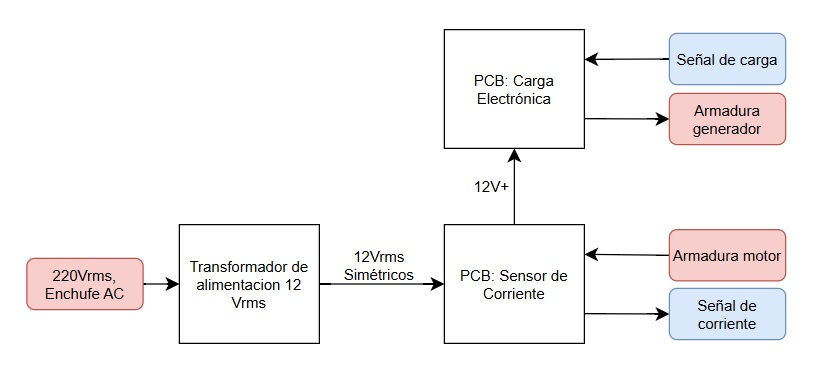
\includegraphics[width=0.7\linewidth]{img//solucion/diagramaSol.jpg}
    \caption{Diagrama de bloques general de la solución}
    \label{fig:dSol}
\end{figure}

En este y en los siguientes diagramas de bloques, los bloques de color rojo corresponden a terminales por los cuales circula una potencia considerable. En cambio, los bloques de color azul representan terminales de señal, asociados a entradas o salidas analógicas de baja corriente.

\subsection{PCB sensor de corriente}

Los diseños de PCB fueron realizados mediante el software EasyEDA y la fabricación de las placas se llevó a cabo en las dependencias del laboratorio de electrónica. Para medir la corriente de armadura del motor, se elaboró una PCB dedicada al acondicionamiento de la señal entregada por el sensor de corriente.

Para explicar el funcionamiento de esta placa electrónica, la Figura \ref{fig:dCorriente} presenta un diagrama de bloques con los circuitos funcionales que la componen.

\begin{figure}[H]
    \centering
    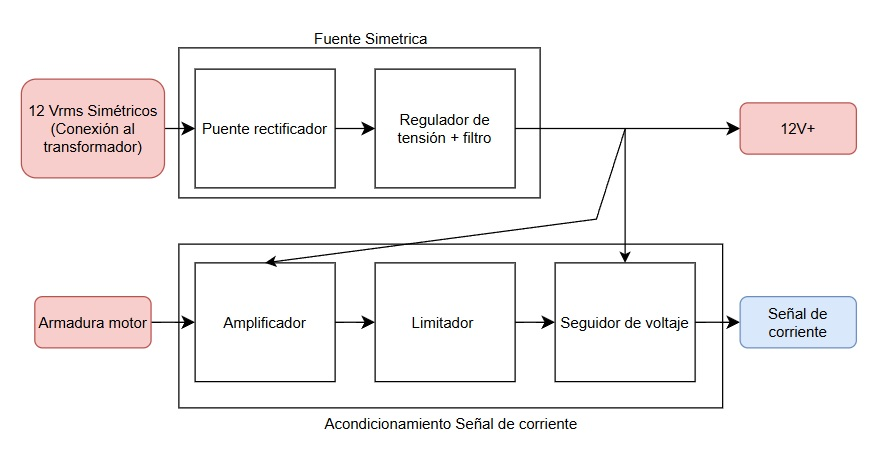
\includegraphics[width=0.7\linewidth]{img//solucion/diagramaCorriente.jpg}
    \caption{Diagrama de bloques de la placa del sensor de corriente}
    \label{fig:dCorriente}
\end{figure}

La Figura \ref{fig:sCorriente} presenta el diagrama esquemático completo del circuito. La corriente de armadura del motor se mide mediante un sensor LA 55-P, mostrado en la Figura \ref{fig:sensor}.

\begin{figure}[H]
    \centering
    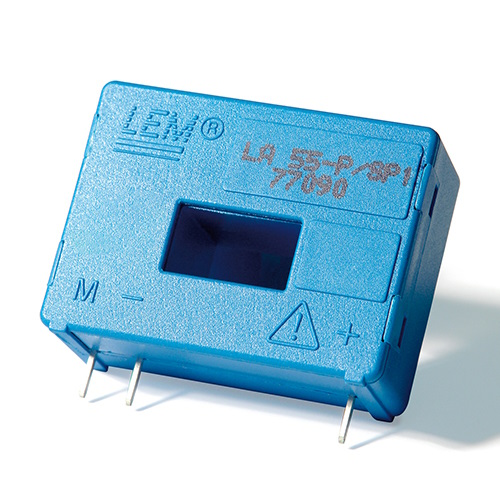
\includegraphics[width=0.4\linewidth]{img//solucion/sensor.jpg}
    \caption{Sensor LA 55-P}
    \label{fig:sensor}
\end{figure}

Para realizar la medición, el cable cuya corriente se desea medir atraviesa la abertura cuadrada del sensor. De esta manera, el dispositivo entrega una corriente proporcional, la cual se transforma en voltaje mediante una resistencia (R3 en el esquemático). Posteriormente, esta señal se amplifica mediante un circuito con amplificadores operacionales, obteniéndose un voltaje de salida de la PCB designado como \texttt{SalidaSensorCorriente}. 

\begin{figure}[H]
    \centering
    
\includegraphics[width=0.75\linewidth]{img//solucion/sensorCorriente1.jpg}
    \caption{Acondicionamiento de la señal de corriente}
    \label{fig:sCorriente}
\end{figure}

Dicho voltaje de salida es una función de la corriente medida y sigue la relación indicada en la Ecuación \ref{eq:Vsalida}.

\begin{equation}
	V_{salidaSensorCorriente} = (1+\frac{R10+R2}{R1}) I_{armadura}' K
	\label{eq:Vsalida}
\end{equation}

Donde las resistencias R2 y R1 son fijas, mientras que R10 es variable y permite ajustar la ganancia de amplificacion, por otro lado, $K$ es una constante de transformacion que depende del sensor LA 55-P y que es desconocida, pero que gracias a la resistencia variable R10, es posible compensarla para que la señal $V_{salidaSensorCorriente}$ posea valores de amplitud entre 0 y 5 V en conjunto con la actuacion del limitador de corriente que no permite que la señal $V_{salidaSensorCorriente}$ sobrepase los 5 V pudiendo dañar las siguientes etapas.\\

%conexion a opto 22 puerto
En cuanto a la conexión con el módulo Ethernet OPTO-22, esta señal de 2 cables (Señal y GND) se conecta a las borneras externas del módulo de entradas analógicas SNAP-AIV-4 (Modulo del OPTO-22)como se muestra a continuación (Figura \ref{fig:snapAivP}).

\begin{figure}[H]
    \centering
    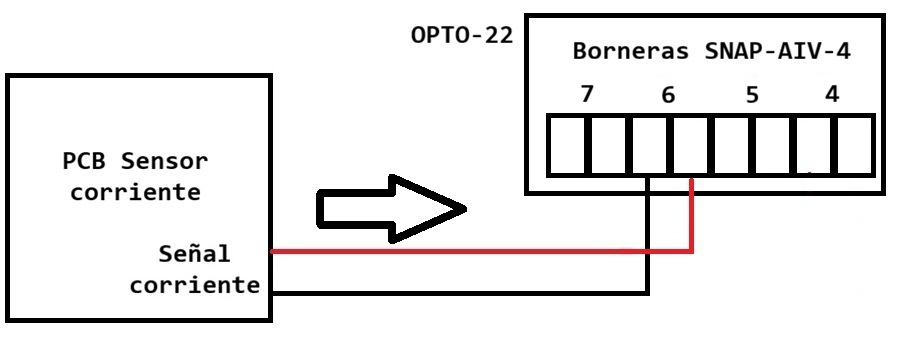
\includegraphics[width=0.75\linewidth]{img//solucion/conexionOPTO22.jpg}
    \caption{Conexión de la señal de corriente al OPTO-22}
    \label{fig:snapAivP}
\end{figure}

La Figura \ref{fig:snapAivR} muestra la conexión física correspondiente.

\begin{figure}[H]
    \centering
    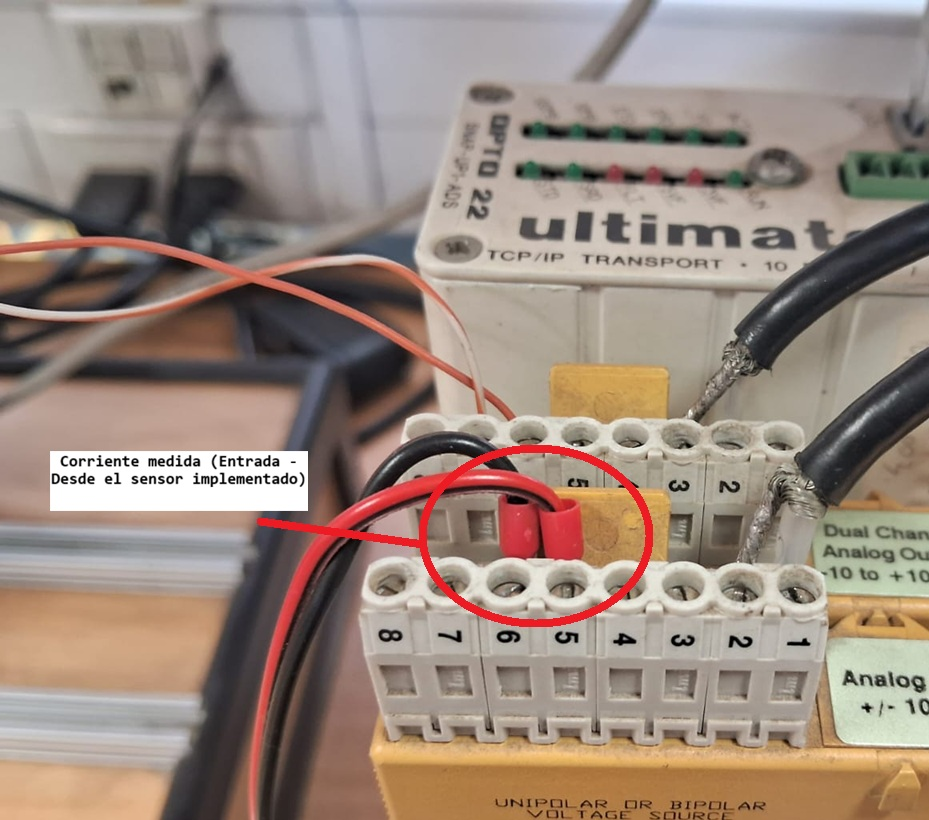
\includegraphics[width=0.4\linewidth]{img//solucion/conexionOPTO22R.jpg}
    \caption{Conexión física de la señal de corriente al OPTO-22}
    \label{fig:snapAivR}
\end{figure}

%recuperacion en simulink 

Hecho esto, la señal es digitalizada dentro del módulo OPTO-22 y enviada a Simulink mediante protocolo Ethernet. En el computador, la señal es recuperada mediante el bloque S-Function \texttt{SDCMotor}, explicado en las secciones anteriores, el cual entrega la medición como una salida en formato \emph{single} (variable \texttt{float} de 32 bits). Para que la señal represente el valor real de la corriente de armadura del motor, se aplica un bloque de ganancia a la salida de la S-Function, como se muestra en la Figura \ref{fig:corrienteSimulink}.

\begin{figure}[H]
    \centering
    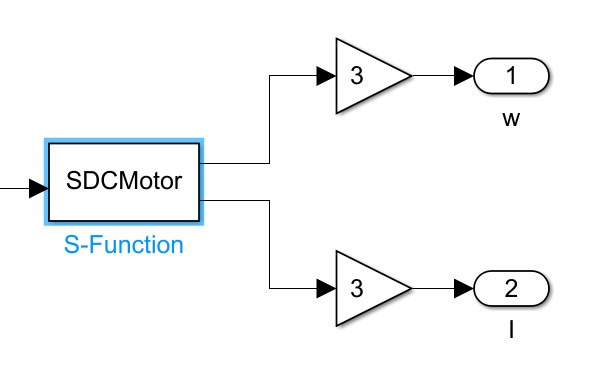
\includegraphics[width=0.4\linewidth]{img//solucion/CorrienteSimulinkSDCMotor.jpg}
    \caption{Recepción de la corriente en Simulink}
    \label{fig:corrienteSimulink}
\end{figure}

En la Figura \ref{fig:corrienteSimulink} se aprecia que la ganancia está establecida en 3. Sin embargo, este valor debe calibrarse mediante mediciones con una fuente de corriente controlada aplicada a la entrada del sensor de corriente. A priori, la ganancia de compensación debería seguir la relación indicada en la Ecuación \ref{eq:Kcompensacion}.

\begin{equation}
	K_{Compensacion} = \frac{1}{(1+\frac{R10+R2}{R1}) K}
	\label{eq:Kcompensacion}
\end{equation}

Donde \(K\) es la ganancia del sensor mencionada anteriormente. Este valor debe determinarse aplicando una corriente conocida en la entrada del sensor y observando el valor medido en Simulink para realizar el despeje correspondiente.\\

Por último, para realizar las funciones de acondicionamiento de la señal de corriente, el circuito requiere una fuente de alimentación simétrica, como se muestra en la Figura \ref{fig:fSimetrica}. El voltaje de salida de la fuente es de \(\pm 12\) VDC.

\begin{figure}[H]
    \centering
    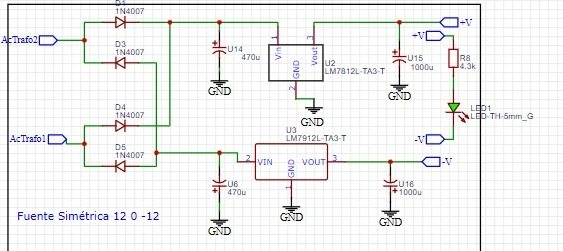
\includegraphics[width=0.75\linewidth]{img//solucion/fuenteSim.jpg}
    \caption{Fuente simétrica}
    \label{fig:fSimetrica}
\end{figure}


\subsection{PCB carga electrónica}

En esta sección se explica el diseño y funcionamiento del circuito implementado como carga electrónica controlada por voltaje. El propósito de este circuito es ofrecer una condición de carga para la armadura del generador, de modo que este ejerza un torque sobre el motor DC. Además, la carga puede ser controlada desde el computador que ejecuta el sistema de control.



Al igual que para el sensor de corriente, se presenta un diagrama de bloques de la estructura funcional de este circuito (Figura \ref{fig:dCarga}).

\begin{figure}[H]
    \centering
    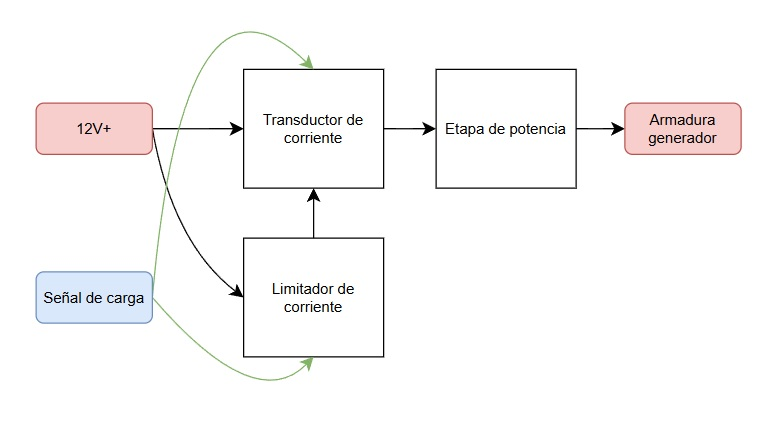
\includegraphics[width=0.7\linewidth]{img//solucion/diagramaCargaElec.jpg}
    \caption{Diagrama de bloques de la carga electrónica}
    \label{fig:dCarga}
\end{figure}

Para entender el funcionamiento del circuito, se debe considerar que el componente principal es el transistor BJT TIP41C. Este componente disipa la mayor parte de la potencia eléctrica generada por el generador, por lo que debe montarse sobre un disipador térmico adecuado. El esquemático de la carga electrónica se muestra en la Figura \ref{fig:cargaElec}.

\begin{figure}[H]
    \centering
    
\includegraphics[width=0.75\linewidth]{img//solucion/cargaElec.jpg}
    \caption{Esquemático carga electrónica}
    \label{fig:cargaElec}
\end{figure}

El circuito se alimenta con 12 V y el transistor se conecta a la armadura del generador. Para controlar la corriente, el módulo recibe un voltaje de entrada denominado \(V_{control}\). Este voltaje se aplica al amplificador operacional, el cual actúa sobre la resistencia R3 indicada en el esquemático de la Figura \ref{fig:cargaElec}. De esta manera, se produce una corriente aproximada igual a \(\frac{V_{control}}{R3}\).

Se utiliza una resistencia \(R3 = 1~\Omega\) para obtener una relación directa entre el voltaje de control y la corriente de carga, es decir, \(iLoad \approx V_{control}\). El transistor TIP41C es el encargado de conducir la corriente que circula por la resistencia, mientras que el amplificador operacional actúa como controlador y no disipa una potencia significativa. En esta implementación es importante utilizar el modelo LM358.

La carga cuenta con dos protecciones principales. En primer lugar, los diodos D2 y D1 evitan daños en el transistor ante una conexión de polaridad inversa. En segundo lugar, el amplificador operacional 1.1 limita el voltaje aplicado sobre la resistencia R3, evitando que la carga solicite una corriente excesiva. El límite de corriente puede ajustarse manualmente mediante el potenciómetro R7.

Para evaluar el desempeño térmico inicial, se realizaron pruebas a distintos voltajes y corrientes, utilizando un sensor de temperatura en el disipador para monitorear la temperatura del transistor TIP41C. Los resultados se presentan en la Tabla \ref{tab:datos}. \\

\textbf{Datos de la prueba}:
\begin{itemize}
	\item Tiempo de funcionamiento: 1 minuto
	\item Temperatura ambiente: 28 grados Celsius.
\end{itemize}

\begin{table}[H]
    \centering
    \caption{Temperaturas medidas (grados Celsius)}
    \begin{tabular}{|c|c|c|c|c|}
        \hline
        V, I & 0.2 A & 0.4 A & 0.6 A &  0.8 A\\
        \hline
        5 V & 28 & 29 & 31 & 30 \\
        \hline
        9 V & 29 & 31 & 33 & 34 \\
        \hline
        12 V & 32 & 33 & 38 & 37 \\
        \hline
    \end{tabular}
    \label{tab:datos}
\end{table}

Para realizar la conexión al módulo OPTO-22, se sigue el diagrama mostrado en la Figura \ref{fig:snapAivCarga}.

\begin{figure}[H]
    \centering
    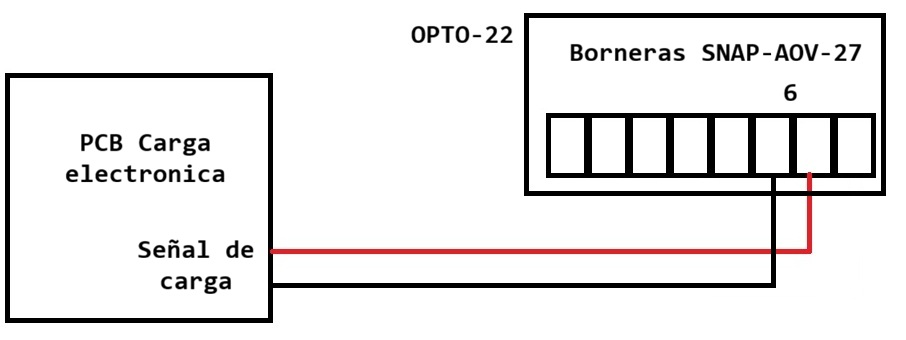
\includegraphics[width=0.7\linewidth]{img//solucion/conexionOPTO22Carga.jpg}
    \caption{Conexión de la señal de carga al OPTO-22}
    \label{fig:snapAivCarga}
\end{figure}

La conexión física correspondiente se muestra en la Figura \ref{fig:snapAivRCarga}.

\begin{figure}[H]
    \centering
    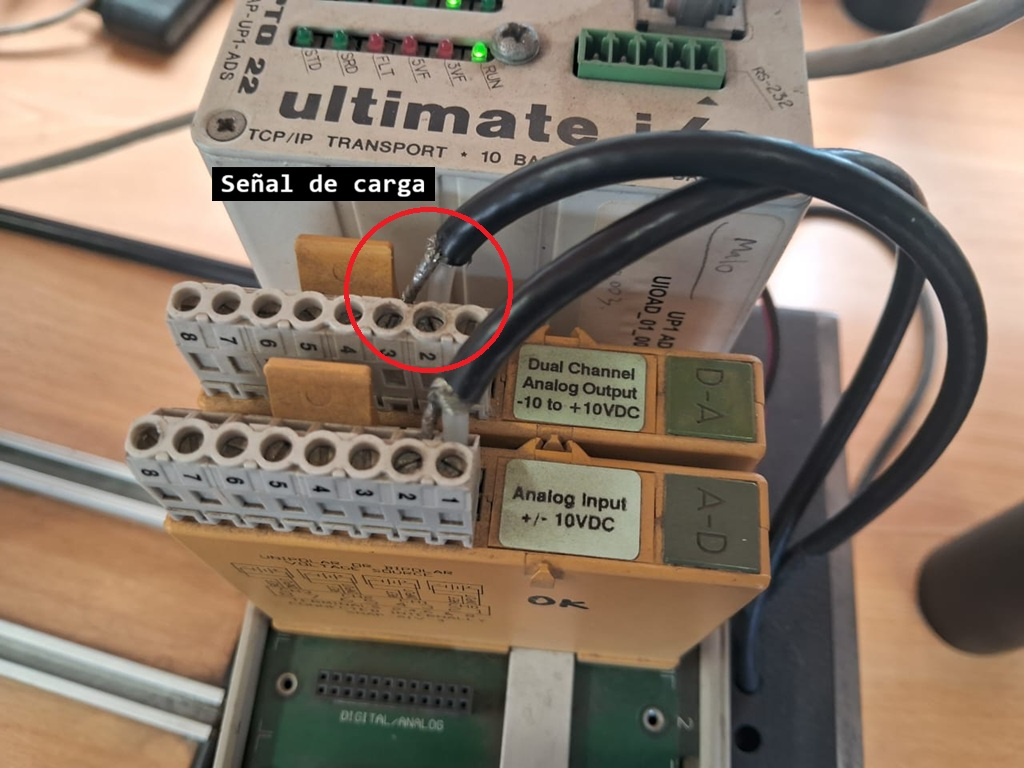
\includegraphics[width=0.5\linewidth]{img//solucion/conexionOPTO22RCarga.jpg}
    \caption{Conexión física de la señal de carga al OPTO-22}
    \label{fig:snapAivRCarga}
\end{figure}



\subsection{Alimentación}

Como se observa en la Figura \ref{fig:dSol}, el dispositivo se alimenta directamente desde la red de 220 VAC. Esta alimentación se adapta mediante la fuente interna y el transformador incorporado en el sistema.\\